\chapter{DASAR TEORI}
Pada bab ini akan dijelaskan mengenai dasar teori yang menjadi dasar pengerjaan Tugas Akhir ini.

\section{\quad Deskripsi Umum Permasalahan}
\quad Permasalahan yang diangkat pada Tugas Akhir ini adalah mencari \textit{Longest Increasing Subsequence} (LIS) dari sebuah \textit{tree}, dimana \textit{node} dalam \textit{tree} tersebut sesuai dengan masukan yang diberikan, dan terdapat \textit{edge} yang saling menghubungkannya. Contoh masukan yang diberikan pada daring terlihat pada Tabel \ref{tabel:cont1}.

\begin{table}[H]
\centering
	\begin{tabular}{|p{2cm}|p{2cm}|}
		\hline
		2\\
		\hline
		12\\
		\hline
		1 8\\
		\hline
		8 6\\
		\hline
		8 3\\
		\hline
		3 12\\
		\hline
		3 10\\
		\hline
		3 5\\
		\hline
		5 4\\
		\hline
		5 2\\
		\hline
		1 9\\
		\hline
		9 11\\
		\hline
		9 7\\
		\hline
	\end{tabular}
	\caption{Contoh masukan dari daring \label{tabel:cont1}}
\end{table}
\quad Dari masukan tadi akan terbentuk sebuah \textit{tree} sesuai seperti angka yang telah dimasukan, visualisasi dari \textit{tree} dapat dilihat di Gambar \ref{fig:treedes}.

\begin{figure}[H]
	\centering
	\begin{tikzpicture}[level/.style={sibling distance = 5cm/#1, level distance = 1.5cm}, scale=0.68,transform shape]
	\node[treenode]{1}
	child{
		node[treenode]{8}
		child{
			node[treenode]{6}
		}
		child{
			node[treenode]{3}
			child{
				node[treenode]{12}
			}
			child{
				node[treenode]{10}
			}
			child{
				node[treenode]{5}
				child{
					node[treenode]{4}
				}
				child{
					node[treenode]{2}
				}
			}	
		}
	}
	child{
		node[treenode]{9}
		child{
			node[treenode]{11}
		}
		child{
			node[treenode]{7}
		}	
	};
	\end{tikzpicture}
	\caption{Bentuk akhir tree sesuai masukan dari daring\label{fig:treedes}}
\end{figure}
\quad Dari \textit{tree} tersebut akan dicari LIS sesuai dengan permasalahan soal, untuk contoh masukan tersebut keluaran LIS adalah $4$. Visualisasi jawaban terlihat pada Gambar \ref{fig:ansex}.

\begin{figure}[H]
	\centering
	\begin{tikzpicture}[level/.style={sibling distance = 5cm/#1, level distance = 1.5cm}, scale=0.68,transform shape]
	\node[treenode]{1}
	child{
		node[treenode,fill=green]{8}
		child{
			node[treenode]{6}
		}
		child{
			node[treenode,fill=green]{3}
			child{
				node[treenode]{12}
			}
			child{
				node[treenode]{10}
			}
			child{
				node[treenode]{5}
				child{
					node[treenode]{4}
				}
				child{
					node[treenode,fill=green]{2}
				}
			}	
		}
	}
	child{
		node[treenode,fill=green]{9}
		child{
			node[treenode,fill=green]{11}
		}
		child{
			node[treenode]{7}
		}	
	};
	\end{tikzpicture}
	\caption{\textit{Vertex} dengan warna hijau menunjukkan \textit{node} yang menjadi anggota LIS.\label{fig:ansex}}
\end{figure}


\section{\quad \textit{Longest Increasing Subsequence}}
\quad Dalam ilmu komputer, permasalahan \textit{Longest Increasing Subsequence} atau yang biasa disingkat menjadi LIS, merupakan permasalahan yang bertujuan untuk menemukan \textit{subsequence} terpanjang dari sebuah \textit{sequence} dimana \textit{subsequence} tersebut memiliki elemen yang sudah disortir dari nilai terkecil ke terbesar.\\
Untuk dapat menyelesaikannya algoritma yang dibutuhkan adalah sebagai berikut:

\quad Dimisalkan terdapat sebuah \textit{array} bernama $A[]$ yang memiliki panjang tertentu, dan penulis juga memiliki LIS terpanjang sementara atau disebut \textit{active list} dengan panjang tertentu. Kemudian penulis ingin menambahkan elemen ke-\textit{i} atau $A[\textit{i}]$ maka harus memperhatikan beberapa hal sebagai berikut\cite{LIS}:
\begin{enumerate}
	\item jika $A[\textit{i}]$ adalah elemen terkecil dari \textit{active list} maka buat \textit{active list} baru dengan panjang $1$.
	\item Jika $A[\textit{i}]$ adalah elemen terbesar dari \textit{active list} maka lakukan duplikasi terhadap \textit{active list} terpanjang dan tambahkan elemen tersebut di akhir.
	\item Jika $A[\textit{i}]$ bukan elemen terbesar ataupun terkecil maka cari \textit{active list} dengan elemen terakhir yang terbesar dan lebih kecil dari $A[\textit{i}]$, lakukan duplikasi dan tambahkan elemen tersebut, dan hapus \textit{list} lain dengan panjang yang sama.
\end{enumerate}
\textbf{Contoh}\\
Untuk menemukan LIS dari array $A[0,8,4,12,2,10,14]$
\begin{enumerate}
	\item $A[0]$ = $1$, karena merupakan elemen pertama dan belum ada \textit{active list} maka masuk ke \textit{case} 1.\\\\
	$[0]$\\
	\item $A[1]$ = $8$, karena angka $8$ lebih besar daripada $0$, maka masuk ke \textit{case} 2.\\\\
	$[0]$\\
	$[0,8]$\\
	\item $A[2]$ = $4$, karena angka $4$ berada di antara $0$ dan $8$, maka akan masuk ke \textit{case} 3.\\\\
	$[0]$\\
	$[0,4]$\\
	\sout{$[0,8]$} (dihilangkan)\\
	\item $A[3]$ = $12$, karena angka $12$ lebih besar daripada $4$, maka masuk ke \textit{case} 1.\\\\
	$[0]$\\
	$[0,4]$\\
	$[0,4,12]$\\\\
	\item $A[4]$ = $2$, karena angka $2$ berada di antara $0$ dan $12$ maka akan masuk ke \textit{case} 3.\\\\
	$[0]$\\
	$[0,2]$\\
	\sout{$[0,4]$} (dihilangkan)\\
	$[0,4,12]$\\
	\item $A[5]$ = $10$, karena angka $10$ berada di antara $0$ dan $12$ maka akan masuk ke \textit{case} 3.\\\\
	$[0]$\\
	$[0,2]$\\
	$[0,2,10]$\\
	\sout{$[0,4,12]$} (dihilangkan)\\
	\item $A[6]$ = $14$, karena angka $14$ lebih besar daripada $10$ maka akan masuk ke \textit{case} 1.\\\\
	$[0]$\\
	$[0,2]$\\
	$[0,2,10]$\\
	$[0,2,10,14]$\\ merupakan LIS dari array tersebut.
\end{enumerate}

\section{\quad \textit{Binary Tree}}
\quad \textit{Binary Tree} merupakan salah satu jenis struktur data \textit{Tree}, yang memiliki maksimal hanya dua \textit{child} untuk setiap \textit{node} yang ada, kedua \textit{child} tersebut biasa disebut dengan istilah \textit{left child} dan \textit{right child}. Gambar \ref{fig:bt} menunjukkan contoh dari \textit{binary tree}.
\begin{figure}[H]
	\centering
	\begin{tikzpicture}[level/.style={sibling distance = 5cm/#1, level distance = 1.5cm}, scale=0.68,transform shape]
	\node[treenode]{}
	child{
		node[treenode]{}
		child{
			node[treenode]{}
		}
		child{
			node[treenode]{}
		}
	}
	child{
		node[treenode]{}
		child{
			node[treenode]{}
		}
		child{
			node[treenode]{}
		}
	};
	\end{tikzpicture}
	\caption{Visualisasi dari bentuk struktur data \textit{Binary Tree}.}\label{fig:bt}
\end{figure}

\section{\quad \textit{Segment Tree}}
\quad\textit{Segment Tree} merupakan salah satu jenis struktur data yang merepresentasikan suatu nilai yang terhubung dengan suatu jeda atau interval tertentu di dalam \textit{array}\cite{ST}.

\quad Dimisalkan terdapat sebuah struktur data \textit{segment tree} yang menyimpan interval untuk suatu \textit{array} $A[]$ dengan panjang $n$.Maka rumusan algoritma yang dapat digunakan untuk konstruksi \textit{segment tree} sebagai berikut\cite{ST2}:
\begin{enumerate}
	\item Buat node yang berisikan seluruh elemen \textit{array} $A[]$.
	\item Jika elemen di dalam node beranggotakan lebih dari satu, maka buat $2$ \textit{child node} baru yang beranggotakan elemen $A[0,... .,n/2]$ dan $A[(n/2)+1,... .,n]$.
	\item Jika elemen di dalam node hanya beranggotakan 1 elemen maka proses dihentikan.
\end{enumerate}
\quad Pada Gambar \ref{fig:subbentukST1} menunjukkan  \textit{node} yang menyimpan nilai dari seluruh rentang yang ada menjadi \textit{root} dari \textit{segment tree}.
\begin{figure}[H]
	\begin{subfigure}{.5\textwidth}
		\centering
		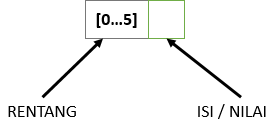
\includegraphics[scale=0.45]{assets/images/pembentukan_ST_1.PNG}
		\caption{}
		\label{fig:subbentukST1}
	\end{subfigure}
	\begin{subfigure}{.5\textwidth}
		\centering
		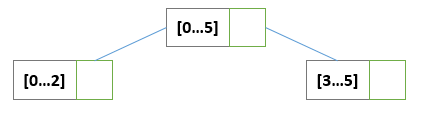
\includegraphics[scale=0.45]{assets/images/pembentukan_ST_2.PNG}
		\caption{}
		\label{fig:subbentukST2}
	\end{subfigure}
	\begin{subfigure}{.5\textwidth}
		\centering 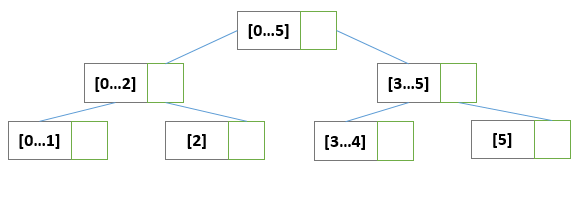
\includegraphics[scale=0.3]{assets/images/pembentukan_ST_3.PNG}
		\caption{}
		\label{fig:subbentukST3}
	\end{subfigure}
		\begin{subfigure}{.5\textwidth}
			\centering
			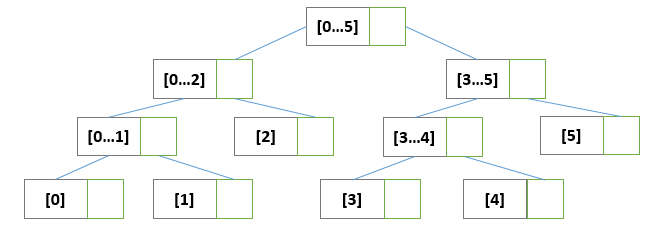
\includegraphics[scale=0.3]{assets/images/pembentukan_ST_4.PNG}
			\caption{}
			\label{fig:subbentukST4}
		\end{subfigure}	
	\caption{Proses pembentukan \textit{Segment Tree}}
	\label{fig:bentukST1}
\end{figure}
\quad Pada Gambar \ref{fig:subbentukST2} menunjukkan proses rekursi untuk membuat dua \textit{child} baru, \textit{child} kiri menyimpan nilai dari rentang 0 hingga 2, \textit{child} kanan menyimpan nilai dari rentang 3 hingga 5.

\quad Pada Gambar \ref{fig:subbentukST3} menunjukkan lanjutan proses rekursi lagi, namun untuk \textit{node} yang menyimpan hanya satu rentang saja, yaitu \textit{node} yang menyimpan rentang 2 dan 5 proses dihentikan, bentuk akhir dari \textit{segment tree} terlihat pada Gambar \ref{fig:subbentukST4}

\quad Selain itu pada umumnya struktur data \textit{segment tree} juga memiliki fungsi \textit{$query()$} untuk mengambil nilai dari suatu rentang dan juga \textit{$update()$} untuk merubah nilai pada suatu rentang.
\quad Algoritma untuk melakukan fungsi \textit{$query()$} sebagai berikut:
\begin{enumerate}
	\item Cek apakah nilai dari rentang yang diinginkan berada dalam rentang saat ini.
	\item Jika iya ambil nilai yang berada di rentang tersebut.
	\item Jika tidak lakukan rekursi ke \textit{left child} dan \textit{right child}.
\end{enumerate}
\quad Untuk visualisasi proses \textit{$query()$} akan diambil nilai pada rentang $1$ sampai $4$. Pada Gambar \ref{fig:subqueryST1} proses dimulai dengan melakukan cek pada \textit{root} apakah rentang yang diinginkan masih termasuk atau tidak, \textit{root} menyimpan nilai dari rentang $0$ hingga $5$, maka rentang yang diinginkan masih termasuk didalamnya, dilakukan proses rekursi ke \textit{child}.
\begin{figure}[H]
	\begin{subfigure}{.5\textwidth}
		\centering
		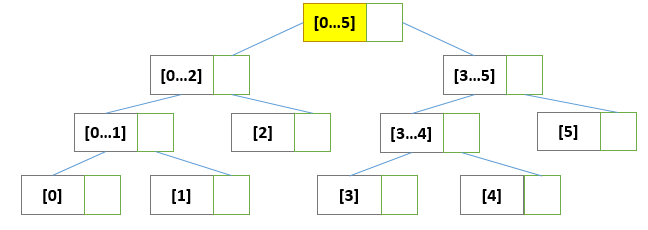
\includegraphics[scale=0.3]{assets/images/Query_ST_1.PNG}
		\caption{}
		\label{fig:subqueryST1}
	\end{subfigure}
	\begin{subfigure}{.5\textwidth}
		\centering
		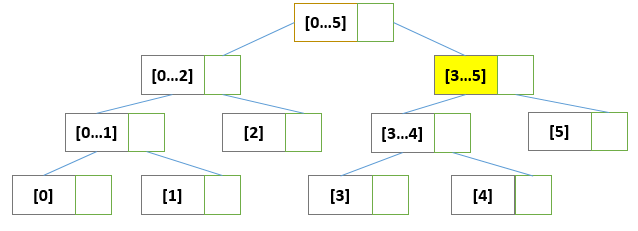
\includegraphics[scale=0.3]{assets/images/Query_ST_2.PNG}
		\caption{}
		\label{fig:subqueryST2}
	\end{subfigure}
	\begin{subfigure}{.5\textwidth}
		\centering 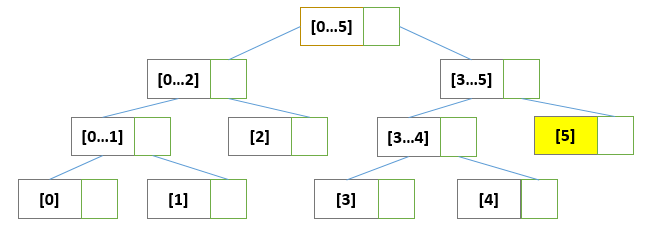
\includegraphics[scale=0.3]{assets/images/Query_ST_3.PNG}
		\caption{}
		\label{fig:subqueryST3}
	\end{subfigure}
	\begin{subfigure}{.5\textwidth}
		\centering
		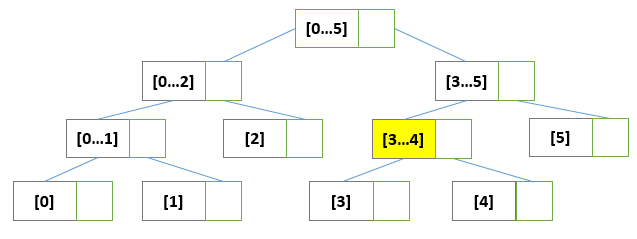
\includegraphics[scale=0.3]{assets/images/Query_ST_4.PNG}
		\caption{}
		\label{fig:subqueryST4}
	\end{subfigure}	
	\caption{Proses rekursi \textit{$query$} pada \textit{right child} dari \textit{Segment Tree} }
	\label{fig:queryST1}
\end{figure}
\quad Pada Gambar \ref{fig:subqueryST2} dilakukan pengecekan pada \textit{node} yang menyimpan rentang nilai $3$ hingga $5$, karena masih mencakup rentang yang dicari maka dilanjutkan proses rekursi pada \textit{child node} tersebut. 

\quad Pada Gambar \ref{fig:subqueryST3} proses dilakukan pada \textit{node} yang menyimpan rentang nilai $5$ saja, karena rentang tersebut tidak dicari, maka proses pada \textit{node} tersebut dihentikan. Pada Gambar \ref{fig:subqueryST4} dilakukan pengecekan pada \textit{node} yang menyimpan rentang nilai $3$ hingga $4$, dimana \textit{node} tersebut menyimpan nilai sesuai dengan rentang yang diinginkan, maka akan diambil nilainya dan dibandingkan dengan \textit{sibling} dari \textit{node} tersebut, untuk kemudian diambil nilai maksimum atau minimum sesuai kebutuhan.

\quad Rekursi dilanjutkan ke \textit{child} yang berada pada sisi kiri dari \textit{root}. Pada Gambar \ref{fig:subqueryST5} proses dilakukan pada \textit{node} yang menyimpan rentang nilai dari rentang $0$ hingga $2$, dikarenakan rentang tersebut mencakup rentang yang diinginkan didalamnya, maka dilakukan proses rekursi ke \textit{child node} tersebut.
\begin{figure}[H]
	\begin{subfigure}{.5\textwidth}
		\centering
		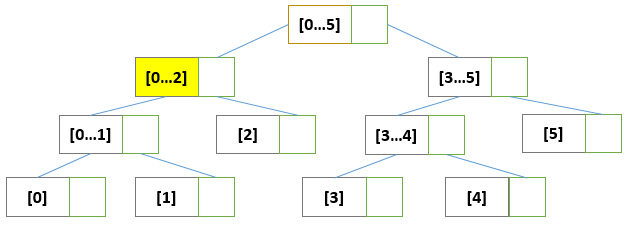
\includegraphics[scale=0.3]{assets/images/Query_ST_5.PNG}
		\caption{}
		\label{fig:subqueryST5}
	\end{subfigure}
	\begin{subfigure}{.5\textwidth}
		\centering
		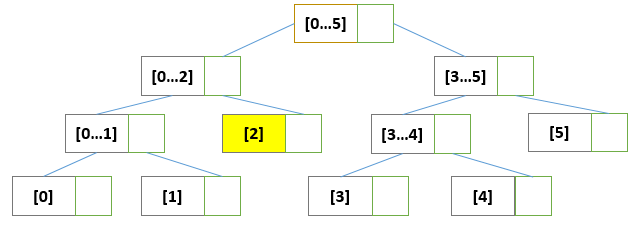
\includegraphics[scale=0.3]{assets/images/Query_ST_6.PNG}
		\caption{}
		\label{fig:subqueryST6}
	\end{subfigure}
	\begin{subfigure}{.5\textwidth}
		\centering 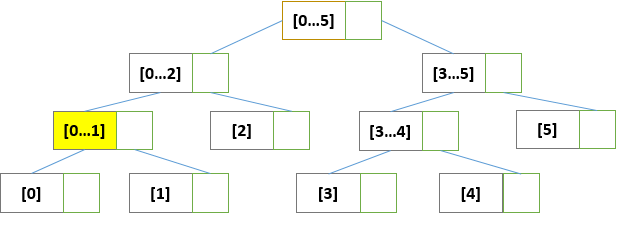
\includegraphics[scale=0.3]{assets/images/Query_ST_7.PNG}
		\caption{}
		\label{fig:subqueryST7}
	\end{subfigure}
	\begin{subfigure}{.5\textwidth}
		\centering
		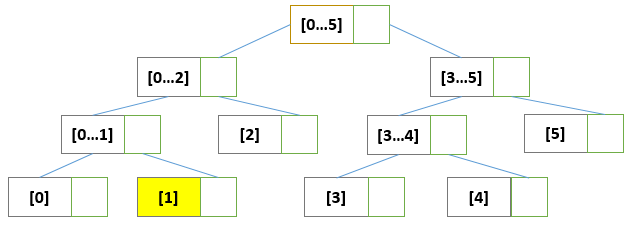
\includegraphics[scale=0.3]{assets/images/Query_ST_8.PNG}
		\caption{}
		\label{fig:subqueryST8}
	\end{subfigure}	
	\caption{Proses rekursi \textit{$query$} pada \textit{left child} dari \textit{Segment Tree}}
	\label{fig:queryST2}
\end{figure}
\quad Pada Gambar \ref{fig:subqueryST6}, karena \textit{node} tersebut termasuk pada rentang yang diinginkan maka nilai didalamnya akan diambil, untuk dibandingkan dengan \textit{sibling} dari \textit{node} tersebut nantinya. Proses dilanjutkan ke \textit{node} yang menyimpan rentang $0$ hingga $1$, seperti pada Gambar \ref{fig:subqueryST7}.

\quad Pada Gambar \ref{fig:subqueryST8} dilakukan pengecekan pada \textit{node} yang menyimpan rentang nilai $1$, dimana \textit{node} tersebut menyimpan nilai sesuai dengan rentang yang diinginkan. Sedangkan pada Gambar \ref{fig:subqueryST9}, nilai pada rentang $0$ tidak termasuk nilai yang diinginkan. 
\begin{figure}[H]
	\begin{subfigure}{.5\textwidth}
		\centering
		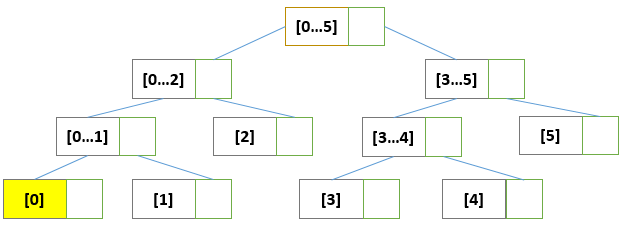
\includegraphics[scale=0.3]{assets/images/Query_ST_9.PNG}
		\caption{}
		\label{fig:subqueryST9}
	\end{subfigure}
	\begin{subfigure}{.5\textwidth}
		\centering
		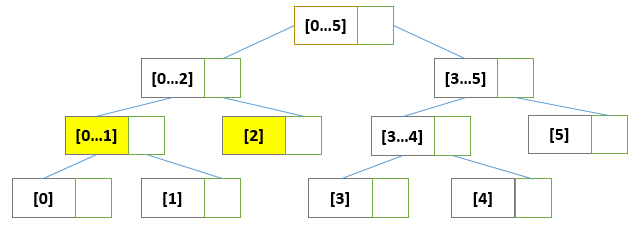
\includegraphics[scale=0.3]{assets/images/Query_ST_10.PNG}
		\caption{}
		\label{fig:subqueryST10}
	\end{subfigure}
	\begin{subfigure}{.5\textwidth}
		\centering 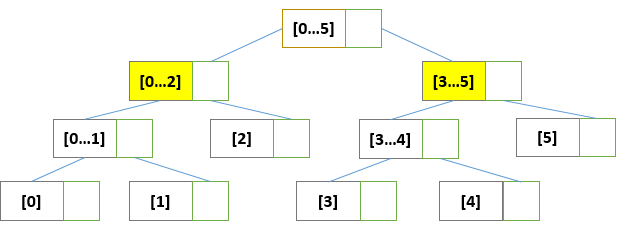
\includegraphics[scale=0.3]{assets/images/Query_ST_11.PNG}
		\caption{}
		\label{fig:subqueryST11}
	\end{subfigure}
	\begin{subfigure}{.5\textwidth}
		\centering
		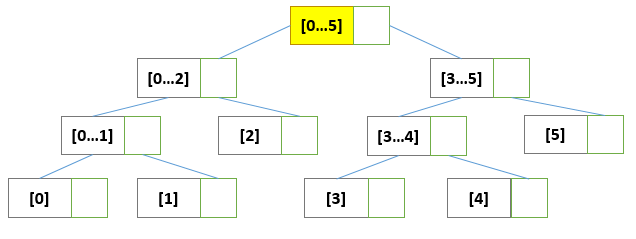
\includegraphics[scale=0.3]{assets/images/Query_ST_12.PNG}
		\caption{}
		\label{fig:subqueryST12}
	\end{subfigure}	
	\caption{Proses pengembalian nilai \textit{$query$} ke \textit{root} pada \textit{Segment Tree}}
	\label{fig:queryST3}
\end{figure}
\quad Sebelum mengembalikan nilai ke atas, akan dilakukan perbandingan nilai, dengan \textit{sibling node} tersebut, untuk mengambil nilai yang maksimum atau minimum sesuai dengan kebutuhan, proses ini terlihat pada Gambar \ref{fig:subqueryST10} dan \ref{fig:subqueryST10}. Pada akhirnya nilai yang dicari akan berada pada \textit{root}, terlihat pada Gambar \ref{fig:subqueryST12}, menandakan bahwa proses \textit{$query()$} telah selesai.
 
\quad Algoritma untuk melakukan fungsi \textit{$update()$} sebagai berikut:
\begin{enumerate}
	\item Cek apakah nilai dari rentang yang diinginkan berada dalam rentang saat ini.
	\item Jika iya ambil \textit{update} nilai yang berada di rentang tersebut.
	\item Jika tidak lakukan rekursi ke \textit{left child} dan \textit{right child}.
\end{enumerate} 
\quad Sebagai contoh akan dilakukan \textit{$update()$} pada \textit{node} yang menyimpan nilai rentang $4$. Awal proses dimulai dengan melakukan pengecekan pada \textit{root}, seperti yang terlihat pada Gambar \ref{fig:subupdateST1}. Karena di dalam \textit{root} mencakup rentang yang ingin diupdate, maka dilakukan rekursi ke \textit{child}.
\begin{figure}[H]
	\begin{subfigure}{.5\textwidth}
		\centering
		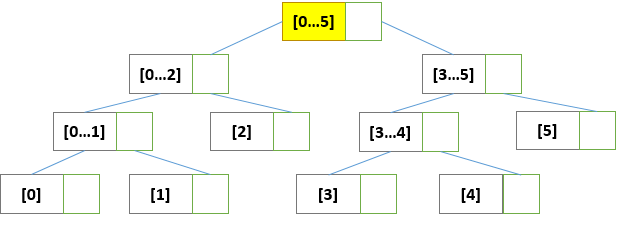
\includegraphics[scale=0.3]{assets/images/Update_ST_1.PNG}
		\caption{}
		\label{fig:subupdateST1}
	\end{subfigure}
	\begin{subfigure}{.5\textwidth}
		\centering
		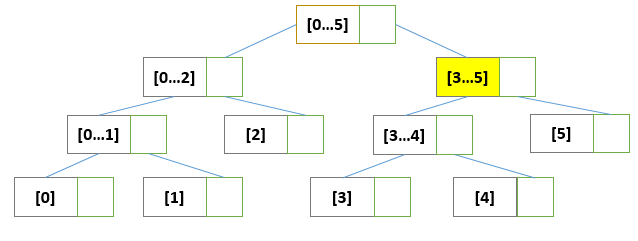
\includegraphics[scale=0.3]{assets/images/Update_ST_2.PNG}
		\caption{}
		\label{fig:subupdateST2}
	\end{subfigure}
	\begin{subfigure}{.5\textwidth}
		\centering
		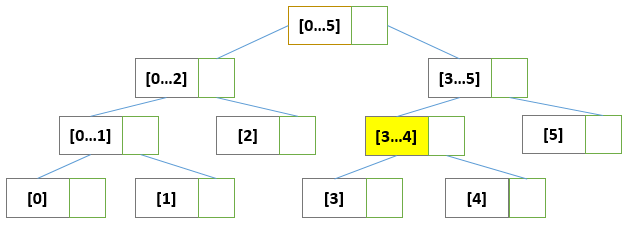
\includegraphics[scale=0.3]{assets/images/Update_ST_3.PNG}
		\caption{}
		\label{fig:subupdateST3}
	\end{subfigure}
	\begin{subfigure}{.5\textwidth}
		\centering
		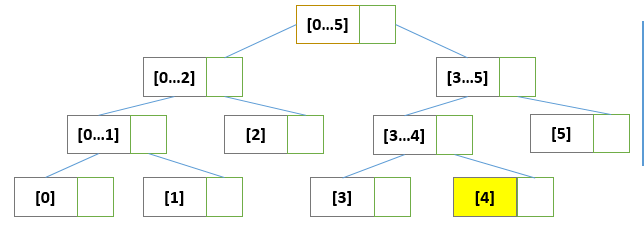
\includegraphics[scale=0.3]{assets/images/Update_ST_4.PNG}
		\caption{}
		\label{fig:subupdateST4}
	\end{subfigure}
	\caption{Proses pencarian \textit{node} untuk melakukan \textit{$update$} pada \textit{Segment Tree}}
	\label{fig:updateST1}
\end{figure}
\quad Karena \textit{left child} dari \textit{root} tidak menyimpan nilai dari rentang yang diinginkan maka proses pada \textit{left child} tidak dilanjutkan. Sedangkan di dalam \textit{right child} dari \textit{root} menyimpan rentang yang diinginkan, maka akan dilakukan rekursi pada \textit{right child}, seperti pada Gambar \ref{fig:subupdateST2}. Pada Gambar \ref{fig:subupdateST3} proses dilanjutkan, karena \textit{node} tersebut masih menyimpan rentang yang diinginkan, maka proses rekursi dilanjutkan ke \textit{child}nya. Pada Gambar \ref{fig:subupdateST4} proses telah mencapai \textit{node} dengan rentang diinginkan, maka akan dilakukan perubahan pada nilai yang disimpan didalamnya. \newpage
\quad Setelah nilai telah diubah, maka sebelum mengembalikan nilai ke \textit{parent}nya akan dilakukan perbandingan nilai dengan \textit{node} yang menjadi \textit{sibling}nya untuk mengambil nilai maksimum atau minimum sesuai dengan kebutuhan, proses ini terlihat pada Gambar \ref{fig:subupdateST5} dan \ref{fig:subupdateST6}, hingga akhirnya nilai kembali pada \textit{root} seperti pada Gambar \ref{fig:subupdateST7}.
\begin{figure}[H]
	\begin{subfigure}{.5\textwidth}
		\centering
		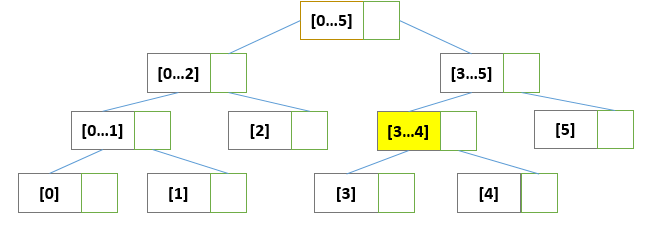
\includegraphics[scale=0.3]{assets/images/Update_ST_5.PNG}
		\caption{}
		\label{fig:subupdateST5}
	\end{subfigure}
	\begin{subfigure}{.5\textwidth}
		\centering
		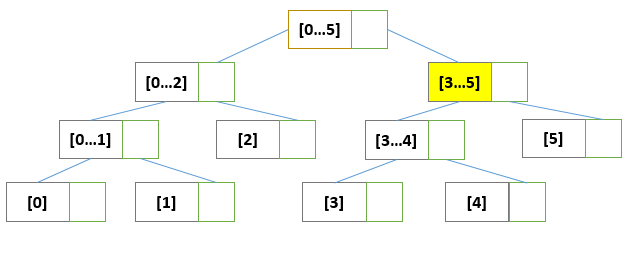
\includegraphics[scale=0.3]{assets/images/Update_ST_6.PNG}
		\caption{}
		\label{fig:subupdateST6}
	\end{subfigure}
	\begin{subfigure}{1.0\textwidth}
		\centering
		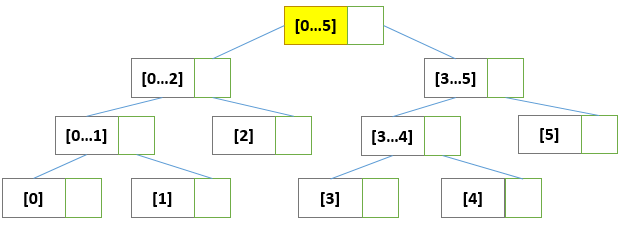
\includegraphics[scale=0.3]{assets/images/Update_ST_7.PNG}
		\caption{}
		\label{fig:subupdateST7}
	\end{subfigure}
	\caption{Proses pengembalian nilai hasil \textit{$update$} pada \textit{Segment Tree}}
	\label{fig:updateST2}
\end{figure}
\section{\quad \textit{Heavy-Light Decomposition}}
\quad\textit{Heavy-Light Decomposition} adalah teknik dekomposisi sebuah \textit{tree} menjadi sebuah \textit{disjoint chains} (tidak ada 2 \textit{chain} yang memiliki \textit{node} yang sama). Disebut \textit{Heavy-Light} karena dekomposisi dilakukan berdasarkan kriteria yang telah ditentukan untuk membedakan apakah \textit{chain} tersebut merupakan \textit{node heavy} atau \textit{light}.

\quad Penggunaan konsep \textit{Heavy-Light Decomposition}, yakni mengumpamakan sebuah \textit{node} mempunyai satu \textit{special child} yang merupakan sebuah \textit{subtree} dengan ukuran paling besar di antara \textit{child} lainnya. sehingga dapat diumpamakan \textit{tree} yang telah dibuat terdiri dari beberapa \textit{chain} dimana setiap \textit{chain} mempunyai \textit{head} yang bukan merupakan \textit{special child} dari \textit{parent child} tersebut.

\quad Setelah membentuk \textit{tree}, selanjutnya dicatat \textit{edge} mana yang merupakan \textit{heavy edge} dan \textit{light edge}. Dengan aturan berikut:
\begin{enumerate}
	\item \textit{Heavy edge} adalah \textit{edge} dengan jumlah \textit{child} lebih besar atau sama dengan setengah jumlah \textit{child} dari \textit{parent child} tersebut.
	\item \textit{Light edge} adalah \textit{edge} dengan jumlah \textit{child} kurang dari setengah jumlah \textit{child} dari \textit{parent child} tersebut.
\end{enumerate}
\quad Pada Gambar \ref{fig:ht} dapat dilihat terdapat banyak warna berbeda, setiap warna menggambarkan \textit{chain} yang berbeda, dan \textit{heavy chain} untuk \textit{tree} tersebut ditandai dengan warna hijau.
\begin{figure}[H]
\centering
\begin{tikzpicture}[level/.style={sibling distance = 5cm/#1, level distance = 1.5cm}, scale=0.68,transform shape]
	\node[treenode,fill=green]{1}
	child{
		node[treenode,fill=green]{2}
		child{
			node[treenode,fill=yellow]{5}
		}
		child{
			node[treenode,fill=green]{6}
			child{
				node[treenode,fill=green]{8}
				child{
					node[treenode,fill=green]{10}
					}
				child{
					node[treenode,fill=brown]{11}
					}
				}
		}
	}
	child{
		node[treenode,fill=cyan]{3}
		child{
			node[treenode,fill=cyan]{7}
			child{
				node[treenode,fill=cyan]{9}
			}
		}
	}
	child{
		node[treenode,fill=pink]{4}
		};
\end{tikzpicture}
\caption{Contoh penggambaran \textit{Heavy-Light Decomposition}\label{fig:ht}}
\end{figure}

\section{\quad \textit{Disjoint Set Union}}
\quad Struktur data \textit{disjoint set} adalah sebuah struktur data yang menyimpan sekumpulan himpunan atau \textit{set}. Dua himpunan bisa disebut \textit{disjoint} jika kedua himpunan tersebut tidak memiliki perpotongan, atau perpotongannya sama dengan $\textit{null}$. Sebagai contoh himpunan $\{1,2\}$ dan $\{3,4\}$ merupakan himpunan yang \textit{disjoint} karena tidak memiliki elemen yang sama diantara keduanya.

\quad \textit{Disjoint set union} sendiri merupakan suatu algoritma yang digunakan untuk menyatukan himpunan yang \textit{disjoint} dengan himpunan lainnya. Hal ini dapat dilakukan dengan melakukan operasi \textit{$merge(a,b)$}, dimana $a$ dan $b$ adalah dua himpunan yang saling \textit{disjoint}.

\textbf{Contoh}:\\
\quad Dimisalkan terdapat $5$ buah himpunan bagian yang memiliki anggota berjumlah $1$ yaitu: $\{1\}$, $\{2\}$, $\{3\}$, $\{4\}$, dan $\{5\}$. Kemudian dilakukan operasi seperti pada Tabel \ref{tabel:visdsu1} dan \ref{tabel:visdsu2}.
\begin{table}[H]
	\begin{tabular}{|p{0.25cm}|p{2.5cm}|p{3.5cm}|p{2.5cm}|}
		\hline
		No & Operasi & Visualisasi Himpunan & Keterangan\\
		\hline
		1 & Kondisi Awal & \centering
		\begin{tikzpicture}
		[level/.style={sibling distance = 1.5cm/#1, level distance = 1.5cm}, scale=0.6,transform shape]
		\node[treenode]{1};
		\addvmargin{10mm}
		\end{tikzpicture}
		\begin{tikzpicture}
		[level/.style={sibling distance = 1.5cm/#1, level distance = 1.5cm}, scale=0.6,transform shape]
		\node[treenode]{2};
		\addvmargin{10mm}
		\end{tikzpicture}
		\begin{tikzpicture}
		[level/.style={sibling distance = 1.5cm/#1, level distance = 1.5cm}, scale=0.6,transform shape]
		\node[treenode]{3};
		\addvmargin{10mm}
		\end{tikzpicture}
		\begin{tikzpicture}
		[level/.style={sibling distance = 1.5cm/#1, level distance = 1.5cm}, scale=0.6,transform shape]
		\node[treenode]{4};
		\addvmargin{10mm}
		\end{tikzpicture}
		\begin{tikzpicture}
		[level/.style={sibling distance = 1.5cm/#1, level distance = 1.5cm}, scale=0.6,transform shape]
		\node[treenode]{5};
		\addvmargin{10mm}
		\end{tikzpicture} & Kondisi awal himpunan.
		\\ \hline
		2 & $merge(2,1)$ & \centering
		\begin{tikzpicture}
		[level/.style={sibling distance = 1.5cm/#1, level distance = 1.5cm}, scale=0.6,transform shape]
		\node[treenode]{1}
		child{
			node[treenode]{2}
		};
		\addvmargin{10mm}
		\end{tikzpicture}
		\begin{tikzpicture}
		[level/.style={sibling distance = 1.5cm/#1, level distance = 1.5cm}, scale=0.6,transform shape]
		\node[treenode]{3};
		\addvmargin{10mm}
		\end{tikzpicture}
		\begin{tikzpicture}
		[level/.style={sibling distance = 1.5cm/#1, level distance = 1.5cm}, scale=0.6,transform shape]
		\node[treenode]{4};
		\addvmargin{10mm}
		\end{tikzpicture}
		\begin{tikzpicture}
		[level/.style={sibling distance = 1.5cm/#1, level distance = 1.5cm}, scale=0.6,transform shape]
		\node[treenode]{5};
		\addvmargin{10mm}
		\end{tikzpicture} & Kondisi setelah $merge(2,1)$.
		\\ \hline
	\end{tabular}\caption{Visualisasi Himpunan bagian dan proses \textit{$merge()$} bagian 1. \label{tabel:visdsu1}}
\end{table}
\hspace{-2cm}
\begin{table}[H]
	\begin{tabular}{|p{0.25cm}|p{2.5cm}|p{3.5cm}|p{2.5cm}|}
		\hline
		3 & $merge(4,3)$ & \centering
		\begin{tikzpicture}
		[level/.style={sibling distance = 1.5cm/#1, level distance = 1.5cm}, scale=0.6,transform shape]
		\node[treenode]{1}
		child{
			node[treenode]{2}
		};
		\addvmargin{10mm}
		\end{tikzpicture}
		\begin{tikzpicture}
		[level/.style={sibling distance = 1.5cm/#1, level distance = 1.5cm}, scale=0.6,transform shape]
		\node[treenode]{3}
		child{
			node[treenode]{4}
		};
		\addvmargin{10mm}
		\end{tikzpicture}
		\begin{tikzpicture}
		[level/.style={sibling distance = 1.5cm/#1, level distance = 1.5cm}, scale=0.6,transform shape]
		\node[treenode]{5};
		\addvmargin{10mm}
		\end{tikzpicture} & Kondisi setelah $merge(4,3)$
		\\ \hline
		4 & $merge(3,1)$ & \centering
		\begin{tikzpicture}
		[level/.style={sibling distance = 1.5cm/#1, level distance = 1.5cm}, scale=0.6,transform shape]
		\node[treenode]{1}
		child{
			node[treenode]{2}
		}
		child{
			node[treenode]{3}
			child{
				node[treenode]{4}
			}
		};
		\addvmargin{10mm}
		\end{tikzpicture}
		\begin{tikzpicture}
		[level/.style={sibling distance = 1.5cm/#1, level distance = 1.5cm}, scale=0.6,transform shape]
		\node[treenode]{5};
		\addvmargin{10mm}
		\end{tikzpicture} & Kondisi setelah $merge(3,1)$
		\\ \hline
		5 & $merge(5,2)$ & \centering
		\begin{tikzpicture}
		[level/.style={sibling distance = 1.5cm/#1, level distance = 1.5cm}, scale=0.6,transform shape]
		\node[treenode]{1}
		child{
			node[treenode]{2}
			child{
				node[treenode]{5}
			}
		}
		child{
			node[treenode]{3}
			child{
				node[treenode]{4}
			}
		};
		\addvmargin{10mm}
		\end{tikzpicture} & Kondisi setelah $merge(5,2)$
		\\ \hline
	\end{tabular}
	\caption{Visualisasi Himpunan bagian dan proses \textit{$merge()$} bagian 2. \label{tabel:visdsu2}}
\end{table}
\section{\quad \textit{Preorder Numbering}}
\quad \textit{Preorder} merupakan salah satu metode \textit{traversing} sebuah \textit{tree}, yang juga merupakan bagian dari algoritma \textit{Depth-First Search} (DFS), yaitu sebuah algoritma yang mencari \textit{depth} atau kedalaman sedalam mungkin pada setiap \textit{child} sebelum melanjutkan ke \textit{sibling} selanjutnya.

\quad Algoritma dari \textit{preorder} adalah sebagai berikut:
\begin{enumerate}
	\item Cek apakah \textit{node} saat ini kosong
	\item Tampilkan nilai/data dari \textit{node} saat ini.
	\item Lakukan \textit{traverse} ke \textit{child} sebelah kiri secara rekursif.
	\item Lakukan \textit{traverse} ke \textit{child} sebelah kanan secara rekursif.
\end{enumerate}
\quad Visualisasi dari \textit{preorder} dapat dilihat pada Gambar \ref{fig:preorder}.
\begin{figure}[H]
	\centering
	\begin{tikzpicture}[level/.style={sibling distance = 5cm/#1, level distance = 1.5cm}, scale=0.68,transform shape]
	\node[treenode]{1}
	child{
		node[treenode]{2}
		child{
			node[treenode]{4}
			}
		child{
			node[treenode]{5}
			}
		}
	child{
		node[treenode]{3}
		};
	\end{tikzpicture}
	\caption{Visualisasi dari \textit{preorder} urutan yang sesuai menjadi 1,2,4,5,3}\label{fig:preorder}
\end{figure}

\section{\quad Permasalahan \textit{LIS and TREE} pada SPOJ}
\quad Pada subbab ini akan dijelaskan mengenai permasalahan yang unik, untuk membuktikkan kebenaran implementasi \textit{disjoint set union} pada struktur data \textit{tree}. Contoh permasalahan tersebut adalah permasalahan pada situs penilaian daring SPOJ dengan judul permasalahan \textit{LIS and TREE} dengan kode soal \textit{LISTREE} deskripsi soal ditunjukkan oleh Gambar \ref{figure:deskripsi}. 
\begin{figure}[H]
	\centerline{ 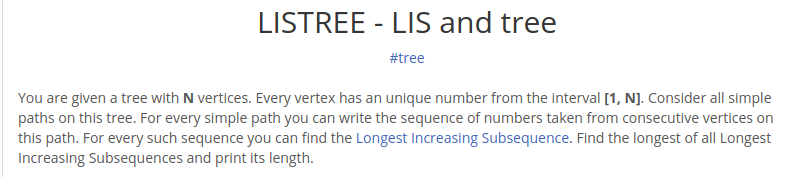
\includegraphics[scale=0.39]{assets/images/deskripsi.png}}
	\caption{Deskripsi soal \textit{LIS and TREE} pada situs penilaian daring SPOJ}
	\label{figure:deskripsi}
\end{figure}
\quad Di dalam soal tersebut dideskripsikan terdapat sebuah \textit{tree} dengan $N$ \textit{node}. Di mana setiap \textit{node} memiliki angka yang unik, dengan interval $1$ sampai $N$. Dalam soal ini di deskripsikan bahwa setiap \textit{path} merupakan \textit{simple path}, yang memiliki arti bahwa tidak ada \textit{node} yang berulang. Untuk setiap \textit{path} dapat dituliskan serangkaian angka yang diambil secara berurutan dari setiap \textit{node}. Untuk setiap rangkaian tersebut dapat dicari LIS nya masing-masing. Tujuan dari soal ini adalah untuk menemukan LIS terpanjang dari semua LIS yang terbentuk dari setiap \textit{path}.

\quad Format masukan diawali dengan sebuah bilangan bulat $T$ dimana $T(1\leq T\leq 1000)$ yang menggambarkan banyaknya \textit{testcase} atau \textit{data sets}. Kemudian untuk setiap $T$ terdapat sebuah bilangan bulat $N$ dimana $N(1\leq N\leq 100000)$ yang merepresentasikan jumlah \textit{node} untuk setiap \textit{testcase} yang nantinya akan membentuk \textit{tree}. Setelah itu terdapat $N-1$ baris dimana terdapat dua bilangan bulat $a$ dan $b$ dimana $(1\leq a,b\leq N)$ yang menunjukkan terdapat sebuah \textit{edge} yang menghubungkan \textit{node} $a$ dan \textit{node} $b$.

\quad Format keluaran berupa sebuah bilangan bulat yang menunjukkan panjang dari LIS terpanjang di antara semua \textit{simple path}. Contoh format masukan dan keluaran dapat dilihat pada Gambar \ref{figure:i/o}. 

\begin{figure}[H]
	\centerline{ 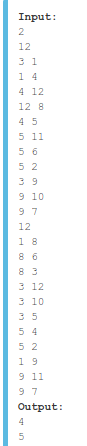
\includegraphics[scale=0.43]{assets/images/input-output.png}}
	\caption{Contoh format masukan pada situs penilaian daring SPOJ}
	\label{figure:i/o}
\end{figure}
\quad Dari contoh format masukkan pada Gambar \ref{figure:i/o} diminta jumlah kasus uji $(T)$ sebanyak $2$, kemudian pada kasus uji kedua diberi masukkan $12$ yang menggambarkan jumlah \textit{node} $(N)$. Kemudian terdapat $11$ baris yang berisikan dua bilangan bulat yaitu $a$ dan $b$, yang mengindikasikan bahwa kedua \textit{node} saling terhubung, dan \textit{node} $a$ menjadi \textit{parent} dari \textit{node} $b$, dimana pada akhirnya akan membentuk sebuah \textit{tree}. Proses pembentukkan tersebut dapat dilihat di Tabel \ref{tabel:visinput1}.
\begin{table}[H]
	\begin{tabular}{|p{0.5cm}|p{2.75cm}|p{3.0cm}|p{2.0cm}|}
		\hline
		No & Masukan $a$ dan $b$ & Bentuk Tree & Keterangan\\
		\hline
		1 & $a$ = 1 $b$ = 8 & \centering
		\begin{tikzpicture}
		[level/.style={sibling distance = 1.5cm/#1, level distance = 1.5cm}, scale=0.6,transform shape]
		\node[treenode]{1}
		child{
			node[treenode]{8}
		};
		\addvmargin{10mm}
		\end{tikzpicture} & Masukan baris ke-1
		\\ \hline
		2 & $a$ = 8 $b$ = 6 & \centering
		\begin{tikzpicture}
		[level/.style={sibling distance = 1.5cm/#1, level distance = 1.5cm}, scale=0.6,transform shape]
		\node[treenode]{1}
		child{
			node[treenode]{8}
			child{
				node[treenode]{6}
				}  
		};
		\addvmargin{10mm}
		\end{tikzpicture} & Masukan baris ke-2
		\\ \hline
		3 & $a$ = 8 $b$ = 3 & \centering
		\begin{tikzpicture}
		[level/.style={sibling distance = 2.5cm/#1, level distance = 1.5cm}, scale=0.6,transform shape]
		\node[treenode]{1}
		child{
			node[treenode]{8}
			child{
				node[treenode]{6}
			}
			child{
				node[treenode]{3}
				}
		};
		\addvmargin{10mm}
		\end{tikzpicture} & Masukan baris ke-3
		\\ \hline
	\end{tabular}\caption{Visualisasi proses pembentukkan \textit{tree} dari masukan pada daring. \label{tabel:visinput1}}
\end{table}

\quad Proses berlanjut hingga masukan terakhir, hingga membentuk \textit{tree} seperti pada Gambar \ref{fig:fulvis}.

\begin{figure}[H]
\centering
\begin{tikzpicture}[level/.style={sibling distance = 5cm/#1, level distance = 1.5cm}, scale=0.68,transform shape]
	\node[treenode]{1}
	child{
		node[treenode]{8}
		child{
			node[treenode]{6}
		}
		child{
			node[treenode]{3}
			child{
				node[treenode]{12}
				}
			child{
				node[treenode]{10}
			}
			child{
				node[treenode]{5}
				child{
					node[treenode]{4}
					}
				child{
					node[treenode]{2}
				}
			}	
		}
	}
	child{
		node[treenode]{9}
		child{
			node[treenode]{11}
			}
		child{
			node[treenode]{7}
		}	
	};
\end{tikzpicture}
\caption{Bentuk akhir tree sesuai masukan ke-2 pada contoh masukan\label{fig:fulvis}}
\end{figure}
\quad Dari contoh masukan kedua di situs penilaian daring SPOJ menunjukkan keluaran LIS yaitu 5, visualisasi untuk jawaban tersebut bisa dilihat di Gambar \ref{fig:ansvis}.
\begin{figure}[H]
	\centering
	\begin{tikzpicture}[level/.style={sibling distance = 5cm/#1, level distance = 1.5cm}, scale=0.68,transform shape]
	\node[treenode]{1}
	child{
		node[treenode,fill=green]{8}
		child{
			node[treenode]{6}
		}
		child{
			node[treenode,fill=green]{3}
			child{
				node[treenode]{12}
			}
			child{
				node[treenode]{10}
			}
			child{
				node[treenode]{5}
				child{
					node[treenode]{4}
				}
				child{
					node[treenode,fill=green]{2}
				}
			}	
		}
	}
	child{
		node[treenode,fill=green]{9}
		child{
			node[treenode,fill=green]{11}
		}
		child{
			node[treenode]{7}
		}	
	};
	\end{tikzpicture}
	\caption{\textit{Vertex} dengan warna hijau menunjukkan LIS dari contoh masukan kedua dari situs penilaian daring SPOJ\label{fig:ansvis}}
\end{figure}

\quad Beberapa batasan yang terdapat pada permasalahan \textit{LIS and TREE} adalah sebagai berikut:
\begin{enumerate}
	\item Besar ukuran berkas masukkan dalam sekali uji maksimal 2 MB.
	\item $(1\leq T\leq 1000)$.
	\item $N(1\leq N\leq 100000)$
	\item $(1\leq a,b\leq N)$
	\item Kombinasi dari node a dan b haruslah unik.
	\item Batas memori: 1536MB
	\item Batas sumber kode 50000B
	\item Batas waktu $ 2 $ detik.	
\end{enumerate}


\section{\quad Penyelesaian Permasalahan \textit{LIS and TREE} pada SPOJ}
\quad Pada subbab ini akan dijelaskan bagaimana menyelesaikan permasalahan \textit{LIS and TREE} dengan penjelasan permasalahan seperti pada subbab sebelumnya.

\quad Sesuai pada deskripsi masalah, dapat diketahui bahwa setiap \textit{node} memiliki \textit{parent} yang telah ditentukan sesuai dengan masukan, sesuai dengan penjelasan pada subbab 2.8.

\quad Untuk mengatasi hal tersebut maka digunakanlah konsep \textit{Disjoint set union} dengan menggunakan \textit{array} $2$ dimensi, sebagai contoh akan digunakan masukan seperti pada Gambar \ref{figure:custominput}.
\begin{figure}[H]
	\centerline{ 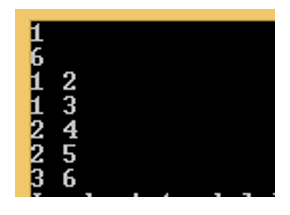
\includegraphics[scale=0.39]{assets/images/Input_contoh.PNG}}
	\caption{Contoh masukan yang digunakan.}
	\label{figure:custominput}
\end{figure}
\quad Visualisasi memasukan masukan pada contoh ke \textit{array} divisualisasikan pada Gambar \ref{figure:olahinput}.
\begin{figure}[H]
	\centerline{ 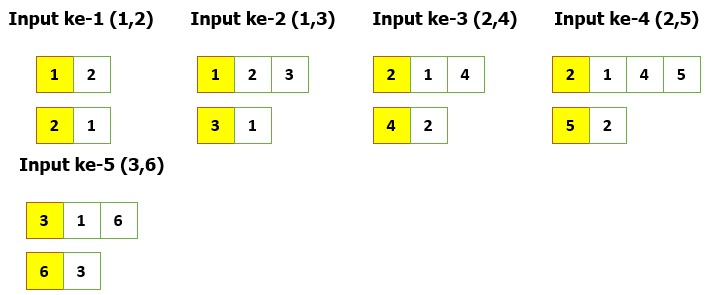
\includegraphics[scale=0.39]{assets/images/Olah_input.PNG}}
	\caption{Visualisasi pengolahan masukan}
	\label{figure:olahinput}
\end{figure}

\quad Dari pengolahan masukan tersebut terlihat bahwa elemen pertama untuk setiap \textit{array} menandakan sebagai \textit{parent} dari \textit{node} tersebut, kecuali untuk \textit{node} $1$ hal ini disebabkan \textit{node} tersebut akan menjadi \textit{root}. Maka dapat terbentuklah \textit{tree} seperti pada Gambar \ref{figure:treeinput}. 
\begin{figure}[H]
	\centerline{ 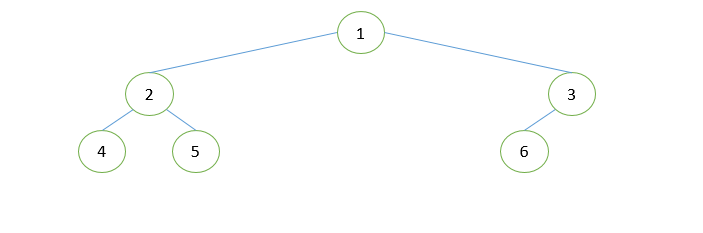
\includegraphics[scale=0.39]{assets/images/Tree_input.PNG}}
	\caption{Visualisasi bentuk \textit{tree} dari contoh masukan}
	\label{figure:treeinput}
\end{figure}
\quad Dalam persoalan \textit{LIS and TREE} LIS yang dicari merupakan sebuah \textit{path} dari \textit{tree} itu sendiri, dan \textit{path} ini merupakan sebuah \textit{simple path} seperti yang telah dijelaskan pada subbab 2.7. Maka untuk mendapatkan nilai LIS tersebut, secara umum terdapat beberapa \textit{case} agar mendapatkan nilai LIS dari setiap \textit{path} yang ada.

\quad \textit{Case} yang ada adalah sebagai berikut:
\begin{enumerate}
	\item \textit{Case} yang pertama adalah jika nilai \textit{node} yang lebih besar berada di atas \textit{node} tersebut, seperti pada Gambar \ref{fig:case1}. Menunjukkan bahwa nilai \textit{node} $a$ > $b$, sehingga arah \textit{path} dari bawah menuju ke atas.
	\item \textit{Case} yang kedua adalah jika nilai \textit{node} yang lebih besar berada di bawah \textit{node} tersebut, seperti pada Gambar \ref{fig:case2}. Menunjukkan bahwa nilai \textit{node} $a$ < $b$, sehingga arah \textit{path} dari atas menuju ke bawah.
	\item \textit{Case} yang kedua adalah jika nilai \textit{node} yang lebih besar berada di \textit{depth} yang sama dari \textit{node} tersebut, seperti pada Gambar \ref{fig:case3}. Menunjukkan bahwa nilai \textit{node} $a$ > $b$, sehingga arah \textit{path} dari bawah menuju ke atas kemudian menuju ke bawah.
\end{enumerate} 
\begin{figure}[H]
	\centering
	\begin{tikzpicture}
		[level/.style={sibling distance = 5cm/#1, level distance = 1.5cm}, scale=0.68,transform shape]
		\node[treenode,fill=green]{a}
		child{
			node[treenode]{}
			child{
				node[treenode]{}
				}
			child{
				node[treenode,fill=green]{b}
				}	
			}
		child{
			node[treenode]{}
			child{
				node[treenode]{}
				}
			child{
				node[treenode]{}
				}
			};
	\end{tikzpicture}\caption{Visualisasi \textit{case} ketika nilai \textit{node child \textgreater parent}.\label{fig:case1}}
\end{figure}
\begin{figure}[H]
	\centering
	\begin{tikzpicture}
	[level/.style={sibling distance = 5cm/#1, level distance = 1.5cm}, scale=0.68,transform shape]
	\node[treenode,fill=green]{a}
	child{
		node[treenode]{}
		child{
			node[treenode,fill=green]{b}
		}
		child{
			node[treenode]{}
		}	
	}
	child{
		node[treenode]{}
		child{
			node[treenode]{}
		}
		child{
			node[treenode]{}
		}
	};
	\end{tikzpicture}\caption{Visualisasi \textit{case} ketika nilai \textit{node parent \textgreater child.}\label{fig:case2}}
\end{figure}
\begin{figure}[H]
	\centering
	\begin{tikzpicture}
	[level/.style={sibling distance = 5cm/#1, level distance = 1.5cm}, scale=0.68,transform shape]
	\node[treenode]{}
	child{
		node[treenode]{}
		child{
			node[treenode,fill=green]{a}
		}
		child{
			node[treenode]{}
		}	
	}
	child{
		node[treenode]{}
		child{
			node[treenode]{}
		}
		child{
			node[treenode,fill=green]{b}
		}
	};
	\end{tikzpicture}\caption{Visualisasi \textit{case} ketika nilai \textit{node} yang lebih besar merupakan \textit{sibling}\label{fig:case3}}
\end{figure}

\quad Untuk dapat menyimpan hasil LIS dari setiap \textit{path} maka diperlukan dua \textit{segment tree} yang akan menyimpan nilai dari tiap interval. \textit{Segment tree} pertama akan menyimpan nilai LIS itu sendiri dan yang kedua akan menyimpan nilai LDS (Longest Decreasing Subsequence) kemudian nantinya jawaban akhir merupakan hasil perbandingan nilai dari dua \textit{segment tree} tersebut.
 
\quad Secara umum algoritma penyelesaian yang dilakukan untuk setiap \textit{node} adalah sebagai berikut:
\begin{enumerate}
	\item Tentukan \textit{child} yang menjadi \textit{big child} atau \textit{small child} menggunakan konsep \textit{Heavy-light Decomposition}.
	\item Lakukan rekursi ke \textit{small child}
	\item Lakukan perulangan untuk mencari LIS dan LDS dari \textit{parent} pada seluruh \textit{child} yang bukan merupakan \textit{bigchild}.
	\item Simpan hasil LIS dan LDS tersebut ke \textit{Segment Tree}.
	\item Cari nilai LIS dan LDS dari \textit{child} ke \textit{parent}.
	\item Simpan hasil LIS dan LDS tersebut ke \textit{Segment Tree}.
	\item Setelah selesai, kembalikan \textit{Segment Tree} ke kondisi semula.
	\item Lakukan rekursi ke \textit{big child}.
	\item Ulangi proses ke 3 hingga 6.
	\item Setelah selesai, biarkan kondisi \textit{Segment Tree} karena akan digunakan kembali.
	\item Lakukan proses hingga semua \textit{node} terlewati.
\end{enumerate}
\quad Proses diawali dari \textit{root} yaitu melakukan pengecekan \textit{child} mana yang merupakan \textit{big} atau \textit{small child} seperti pada Gambar \ref{fig:subproses1}, \ref{fig:subproses2}, dan \ref{fig:subproses3}.
\begin{figure}[H]
	\begin{subfigure}{.5\textwidth}
		\centering
		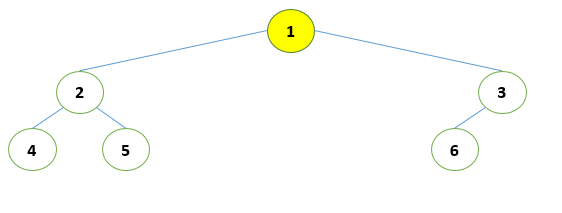
\includegraphics[scale=0.36]{assets/images/Ilustrasi_proses_1.PNG}
		\caption{Memeriksa \textit{child} dari root}
		\label{fig:subproses1}
	\end{subfigure}
	\begin{subfigure}{.5\textwidth}
		\centering
		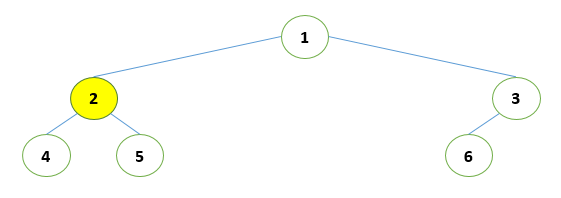
\includegraphics[scale=0.36]{assets/images/Ilustrasi_proses_2.PNG}
		\caption{\textit{Big child} dari \textit{root}}
		\label{fig:subproses2}
	\end{subfigure}
	\begin{subfigure}{.5\textwidth}
		\centering
		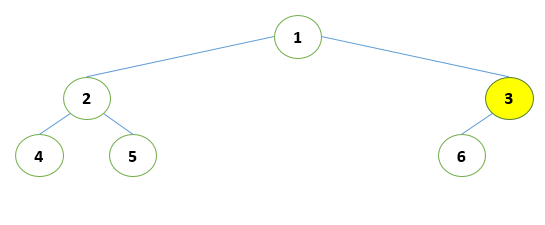
\includegraphics[scale=0.36]{assets/images/Ilustrasi_proses_3.PNG}
		\caption{\textit{Small child} dari \textit{root}}
		\label{fig:subproses3}
	\end{subfigure}
	\begin{subfigure}{.5\textwidth}
		\centering
		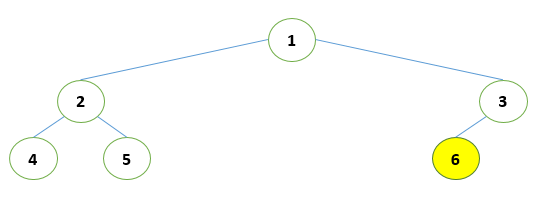
\includegraphics[scale=0.36]{assets/images/Ilustrasi_proses_4.PNG}
		\caption{\textit{Big child} dari \textit{node} 3}
		\label{fig:subproses4}
	\end{subfigure}
	\caption{Penentuan \textit{big child} dan \textit{small child} dari \textit{root}}
	\label{fig:proses1}
\end{figure}

\quad Dari proses sebelumnya diketahui bahwa \textit{small child} dari \textit{root} adalah \textit{node} 3, maka proses akan dilanjutkan pada \textit{node} 3. Pada \textit{node} tersebut dilakukan kembali pencari \textit{big} dan \textit{small child}. Karena hanya memiliki satu \textit{child} saja, maka proses akan langsung dilanjutkan pada \textit{big child}, yaitu \textit{node} 6, ditunjukkan oleh Gambar \ref{fig:subproses4}. 

\quad Pada \textit{node} 6 dilakukan pencarian LIS dan LDS seperti yang tertulis pada algoritma penyelesaian sebelumnya, pada Gambar \ref{fig:proses2} hingga \ref{fig:subproses13} dilakukan proses \textit{$query()$} untuk mencari LIS pada \textit{segment tree} dari rentang $1$ hingga $5$. Proses yang terjadi seperti yang telah dijelaskan pada subbab 2.4.
\begin{figure}[H]
	\vspace{-1.2cm}
	\begin{subfigure}{1.0\textwidth}
		\centering
		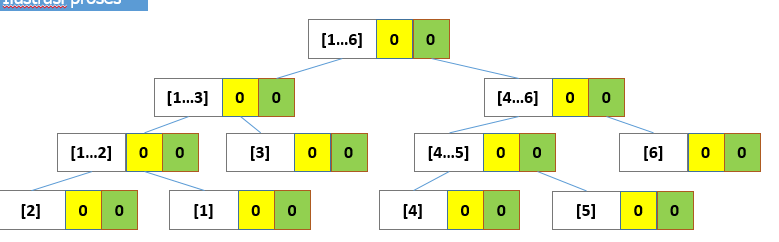
\includegraphics[scale=0.32]{assets/images/Ilustrasi_proses_5.PNG}
		\caption{Kondisi awal \textit{segment tree}}
		\label{fig:subproses5}
	\end{subfigure}
	\begin{subfigure}{1.0\textwidth}
		\centering
		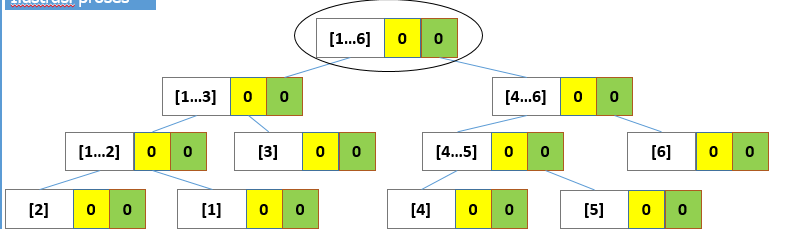
\includegraphics[scale=0.32]{assets/images/Ilustrasi_proses_6.PNG}
		\caption{Memeriksa rentang 1 hingga 6}
		\label{fig:subproses6}
	\end{subfigure}
	\begin{subfigure}{1.0\textwidth}
		\centering
		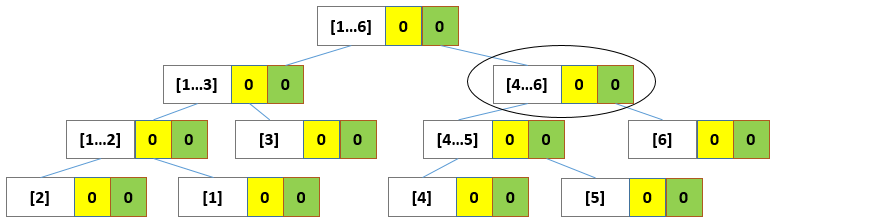
\includegraphics[scale=0.32]{assets/images/Ilustrasi_proses_7.PNG}
		\caption{Memeriksa rentang 4 hingga 6}
		\label{fig:subproses7}
	\end{subfigure}
	\begin{subfigure}{1.0\textwidth}
		\centering
		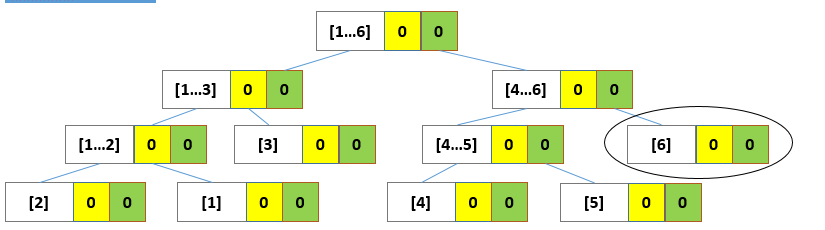
\includegraphics[scale=0.32]{assets/images/Ilustrasi_proses_8.PNG}
		\caption{\textit{Out of range}}
		\label{fig:subproses8}
	\end{subfigure}
	\begin{subfigure}{1.0\textwidth}
		\centering
		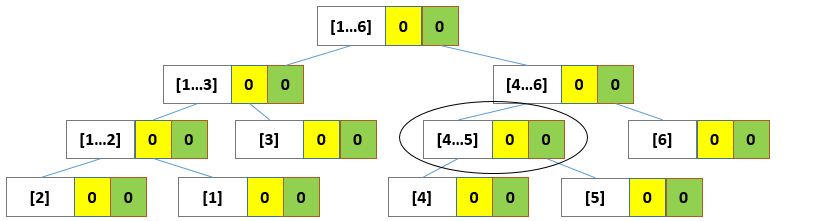
\includegraphics[scale=0.32]{assets/images/Ilustrasi_proses_9.PNG}
		\caption{Mengambil nilai rentang 4 hingga 5}
		\label{fig:subproses9}
	\end{subfigure}
	\begin{subfigure}{1.0\textwidth}
		\centering
		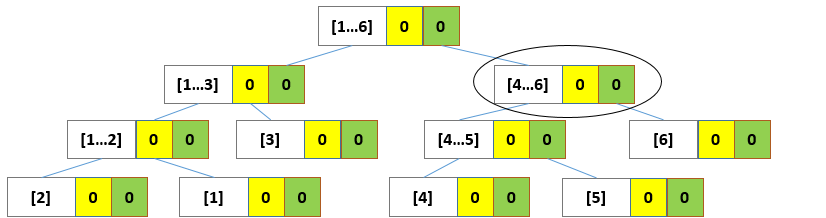
\includegraphics[scale=0.32]{assets/images/Ilustrasi_proses_10.PNG}
		\caption{Mengembalikan nilai ke atas}
		\label{fig:subproses10}
	\end{subfigure}
	\caption{Proses \textit{$query$} nilai LIS \textit{node} 6 pada \textit{right child} dari \textit{segment tree}}
	\label{fig:proses2}
\end{figure}
\begin{figure}[H]
	\begin{subfigure}{1.0\textwidth}
		\centering
		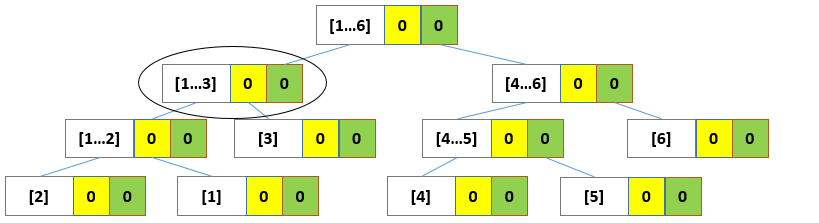
\includegraphics[scale=0.33]{assets/images/Ilustrasi_proses_11.PNG}
		\caption{Mengambil nilai rentang 1 hingga 3}
		\label{fig:subproses11}
	\end{subfigure}
	\begin{subfigure}{1.0\textwidth}
		\centering
		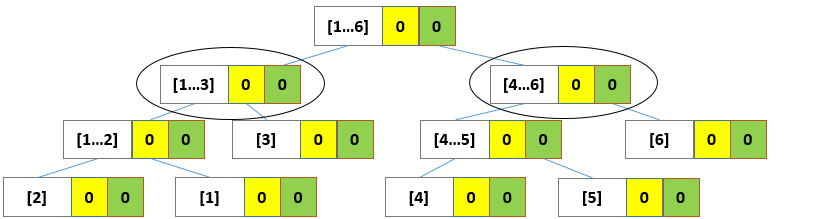
\includegraphics[scale=0.33]{assets/images/Ilustrasi_proses_12.PNG}
		\caption{Membandingkan nilai dengan \textit{sibling}}
		\label{fig:subproses12}
	\end{subfigure}
	\begin{subfigure}{1.0\textwidth}
		\centering
		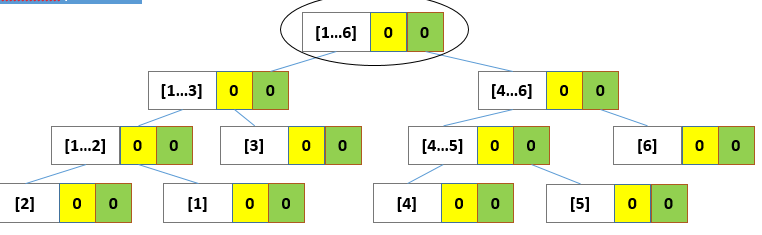
\includegraphics[scale=0.33]{assets/images/Ilustrasi_proses_13.PNG}
		\caption{Mengembalikan nilai ke \textit{root}}
		\label{fig:subproses13}
	\end{subfigure}
	\begin{subfigure}{1.0\textwidth}
		\centering
		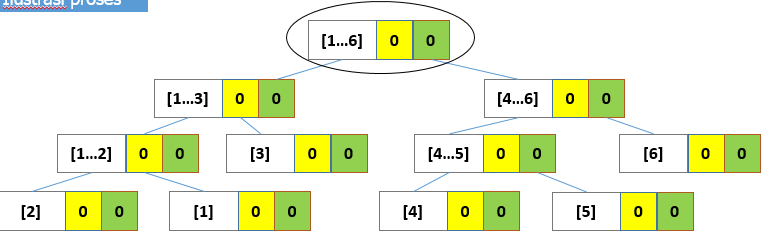
\includegraphics[scale=0.33]{assets/images/Ilustrasi_proses_14.PNG}
		\caption{\textit{Out of range}}
		\label{fig:subproses14}
	\end{subfigure}
	\caption{Proses \textit{$query$} nilai LIS \textit{node} 6 pada \textit{left child} dari \textit{segment tree} dan pengembalian nilai ke \textit{root}}
\end{figure}
\quad Pada Gambar \ref{fig:subproses14} dilakukan pencarian LDS untuk \textit{node} 6, dengan melakukan \textit{$query()$} rentang 7 pada \textit{segment tree}, karena hanya tersedia hingga rentang 6 maka langsung mengembalikan nilai.\newpage

\quad Kemudian hasil \textit{$query()$} disimpan pada variabel sementara milik \textit{node} 6, terlihat pada Gambar \ref{fig:subproses15} nilai LIS dan LDS sementara adalah $1$, maka hasil sementara saat ini adalah $1$.
\begin{figure}[H]
	\begin{subfigure}{1.0\textwidth}
		\centering
		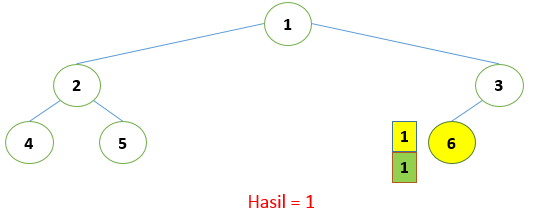
\includegraphics[scale=0.33]{assets/images/Ilustrasi_proses_15.PNG}
		\caption{Kondisi setelah proses \textit{$query$ node} 6}
		\label{fig:subproses15}
	\end{subfigure}
	\begin{subfigure}{1.0\textwidth}
		\centering
		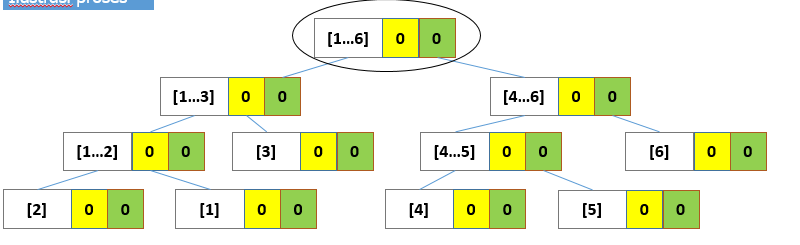
\includegraphics[scale=0.33]{assets/images/Ilustrasi_proses_16.PNG}
		\caption{Memeriksa \textit{root}}
		\label{fig:subproses16}
	\end{subfigure}
	\begin{subfigure}{1.0\textwidth}
		\centering
		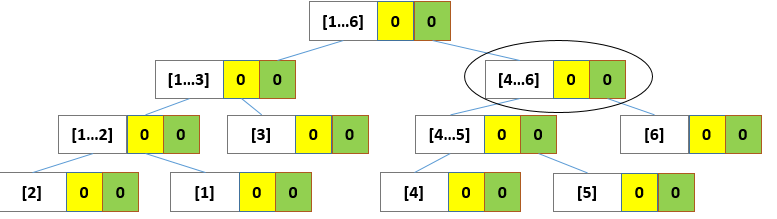
\includegraphics[scale=0.33]{assets/images/Ilustrasi_proses_17.PNG}
		\caption{Memeriksa rentang 4 hingga 6}
		\label{fig:subproses17}
	\end{subfigure}
	\begin{subfigure}{1.0\textwidth}
		\centering
		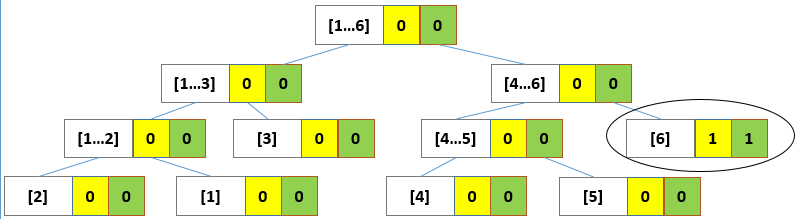
\includegraphics[scale=0.33]{assets/images/Ilustrasi_proses_18.PNG}
		\caption{Memperbarui nilai rentang 6}
		\label{fig:subproses18}
	\end{subfigure}
	\caption{Penyimpanan nilai untuk LIS dan LDS \textit{node} 6 dan \textit{$update()$} pada \textit{segment tree}}
	\label{fig:proses4}
\end{figure}\newpage
\quad Dikarenakan \textit{node} 6 merupakan \textit{big child} maka perlu dilakukan \textit{$update()$} pada \textit{segment tree}, \textit{update} akan dilakukan pada \textit{node} yang menyimpan nilai dari rentang 6. Proses fungsi \textit{$update()$} sendiri seperti yang telah dijelaskan pada subbab 2.4. Gambar \ref{fig:subproses16} hingga Gambar \ref{fig:subproses20}.
\begin{figure}[H]
	\begin{subfigure}{1.0\textwidth}
		\centering
		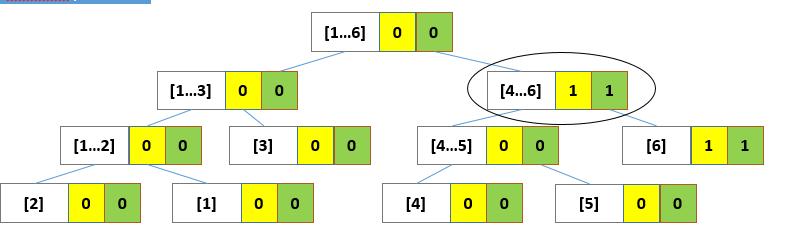
\includegraphics[scale=0.33]{assets/images/Ilustrasi_proses_19.PNG}
		\caption{Mengembalikan nilai ke atas}
		\label{fig:subproses19}
	\end{subfigure}
	\begin{subfigure}{1.0\textwidth}
		\centering
		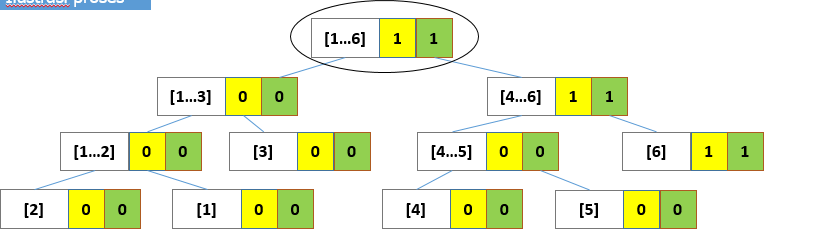
\includegraphics[scale=0.33]{assets/images/Ilustrasi_proses_20.PNG}
		\caption{Mengembalikan nilai ke \textit{root}}
		\label{fig:subproses20}
	\end{subfigure}
	\begin{subfigure}{1.0\textwidth}
		\centering
		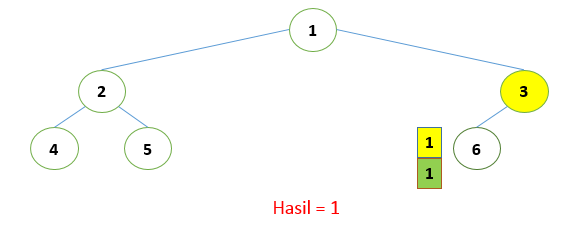
\includegraphics[scale=0.33]{assets/images/Ilustrasi_proses_21.PNG}
		\caption{Melanjutkan proses ke \textit{node} 3}
		\label{fig:subproses21}
	\end{subfigure}
	\caption{Proses \textit{$update()$} pada \textit{segment tree} dan rekursi ke \textit{parent}}
	\label{fig:proses5}
\end{figure}

\quad Proses dilanjutkan ke \textit{parent} dari \textit{node} 6, yaitu \textit{node} 3, divisualkan pada Gambar \ref{fig:subproses21}. Proses yang dilakukan sama yaitu menjalankan \textit{$query()$} untuk mencari nilai LIS dan LDS pada \textit{segment tree}. Nilai yang didapatkan adalah 2 untuk LIS dan LDS, yang disimpan pada variabel sementara milik \textit{node} 3 seperti pada Gambar \ref{fig:subproses22}.
\begin{figure}[H]
	\begin{subfigure}{1.0\textwidth}
		\centering
		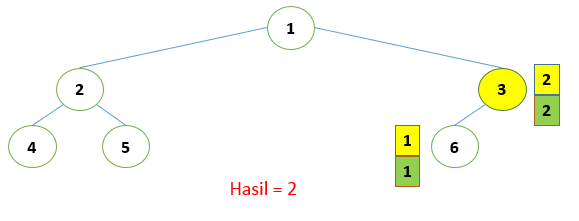
\includegraphics[scale=0.33]{assets/images/Ilustrasi_proses_22.PNG}
		\caption{Kondisi setelah memproses \textit{node} 3}
		\label{fig:subproses22}
	\end{subfigure}
	\begin{subfigure}{1.0\textwidth}
		\centering
		\includegraphics[scale=0.33]{assets/images/Ilustrasi_proses_23.PNG}
		\caption{Kondisi \textit{segment tree} seperti semula}
		\label{fig:subproses23}
	\end{subfigure}
	\begin{subfigure}{1.0\textwidth}
		\centering
		\includegraphics[scale=0.33]{assets/images/Ilustrasi_proses_24.PNG}
		\caption{Kondisi setelah selesai memproses \textit{node} 4 dan 5}
		\label{fig:subproses24}
	\end{subfigure}
	\caption{Pengembalian kondisi \textit{segment tree} seperti semula}
	\label{fig:proses6}
\end{figure}

\quad Karena \textit{node} 3 merupakan \textit{small child}, maka sebelum kembali ke \textit{parent}nya, kondisi \textit{segment tree} perlu dikembalikan seperti semula, yaitu menjadikan seluruh nilai yang ada didalamnya menjadi $0$. Seperti pada Gambar \ref{fig:subproses23}.

\quad Proses dilanjutkan ke \textit{big child} dari \textit{root} yaitu \textit{node} 2 seperti pada Gambar \ref{fig:subproses24}. Tahapan yang dilakukan sama seperti pada \textit{node} 3, dengan mencari \textit{big child} dan \textit{small child} kemudian menyimpan nilai pada variabel sementara untuk setiap \textit{node}. Setelah selesai memproses seluruh \textit{child} dilakukan \textit{query} untuk LIS dan LDS pada \textit{node} 2, dari kondisi \textit{segment tree} seperti pada Gambar \ref{fig:subproses25}, dan akan menyimpan hasilnya pada variabel sementara \textit{node} 2, seperti pada Gambar \ref{fig:subproses26}. Kondisi akhir dari keseluruhan proses ditunjukan oleh Gambar \ref{fig:subproses27} dengan keluaran akhir yaitu $3$.
\begin{figure}[H]
	\begin{subfigure}{1.0\textwidth}
		\centering
		\includegraphics[scale=0.39]{assets/images/Ilustrasi_proses_25.PNG}
		\caption{Kondisi \textit{segment tree} pada \textit{node} 2}
		\label{fig:subproses25}
	\end{subfigure}
	\begin{subfigure}{1.0\textwidth}
		\centering
		\includegraphics[scale=0.39]{assets/images/Ilustrasi_proses_26.PNG}
		\caption{Kondisi setelah proses pada \textit{node} 2}
		\label{fig:subproses26}
	\end{subfigure}
	\begin{subfigure}{1.0\textwidth}
		\centering
		\includegraphics[scale=0.39]{assets/images/Ilustrasi_proses_27.PNG}
		\caption{Kondisi akhir dari keseluruhan proses}
		\label{fig:subproses27}
	\end{subfigure}
	\caption{Proses pencarian LIS dan LDS pada \textit{big child} dari \textit{root} dan pada \textit{root}}
	\label{fig:proses7}
\end{figure}	